\documentclass[aspectratio=169,t,11pt,table]{beamer}
\usepackage{../../slides}
\usepackage{../../math}
\usepackage{../../uark_colors}
\definecolor{accent}{HTML}{9D2235}
\definecolor{accent2}{HTML}{2B5269}

\title{Topic 4: Multiple Regression Analysis}
\subtitle{\it  ECON 4753 — University of Arkansas}
\date{Fall 2024}
\author{Prof. Kyle Butts}

\begin{document}

% ------------------------------------------------------------------------------
\begin{frame}[noframenumbering,plain]
\maketitle

% \bottomleft{\footnotesize $^*$A bit of extra info here. Add an asterich to title or author}
\end{frame}
% ------------------------------------------------------------------------------

\section{Multiple Variable Regression}

\begin{frame}{Multiple Regression}
  The multiple variable linear regression model is written as
  $$
    y_i = \beta_0 + X_{1,i} \beta_1 + \dots + X_{K,i} \beta_K = u_i
  $$
  
  \bigskip
  There are $K$ covariates that we want to \emph{jointly} estimate their associations with $y$
  \begin{itemize}
    \item Note these don't have to be `distinct' variables, but could be polynomials, binned data, interactions between variables, etc. 
  \end{itemize} 
\end{frame}

\begin{frame}{Why Multiple Variable Regression?}{Advertising Example}
  Let's given an example. Say you're a business and you want to use advertising to boost sales. You have a bunch of different markets (e.g. cities) and you have data on how you've spent your advertising budget in those markets and the sales in that market
\end{frame}

\begin{frame}{Advertising Example}{Single-variable predictors}
  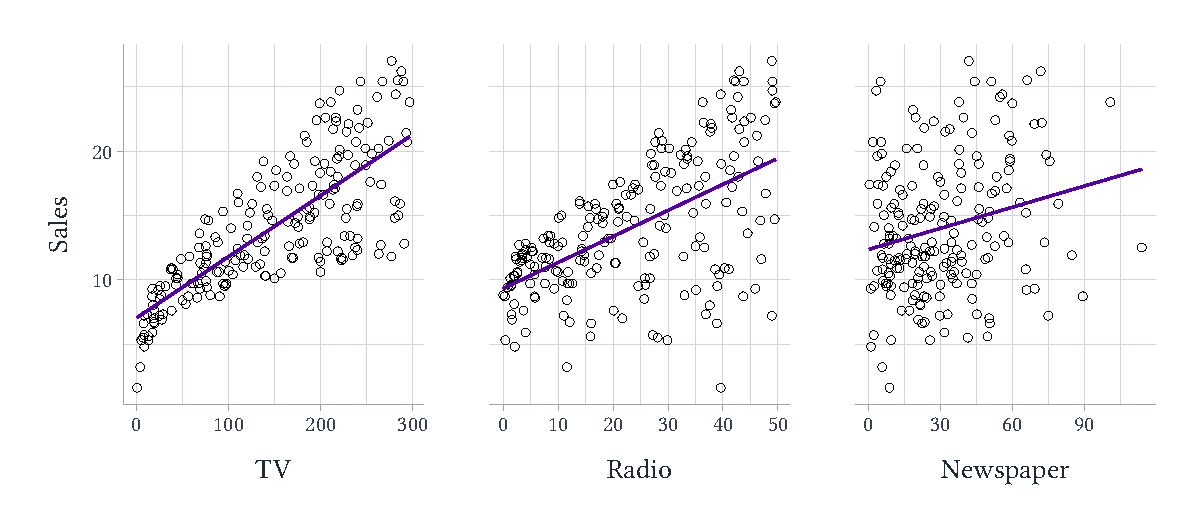
\includegraphics[width=\textwidth]{figures/sales_bivariate.pdf}
\end{frame}

\begin{frame}{Advertising Example}
  We see that sales are higher in markets that have spending on TV, Radio, and Newspaper ads separately. 
  
  \pause
  \bigskip 
  These single scatter plots with line of best-fits are a somewhat poor model:
  \begin{itemize}
    \item Are there synergies between different advertising strategies (are they substitutes or complements to one another)?
    \item Do places with more TV ads also have more radio ads? Then how can we tell if it is TV ads that are helping or if it is really radio ads?
  \end{itemize}

  \pause\bigskip
  \alert{Key takeaway:} Forecasting models get better the more carefully you think about the context you are in
\end{frame}

\begin{frame}{Intuition of multiple linear regression}
  \begin{quote}
    Do places with more TV ads also have more radio ads? Then how can we tell if it is TV ads that are helping or if it is really radio ads ?
  \end{quote}

  \bigskip
  Multiple regression will help with this. To estimate the relationship between sales and radio ads, what we really want to do is compare places with \emph{the same TV ads} but different amounts of radio ads and see how their sales differ

  \pause
  \begin{itemize}
    \item The language typically used by economists is `controlling for TV ads, what is the relationship between radio ads and sales?'
  \end{itemize}
\end{frame}

\begin{frame}{Correlation between $X$}
  More generally, we want to use multiple regression when multiple $X$ variables are correlated with one another. Say $X_{k,i}$ and $X_{\ell,i}$ are correlated with each other.
  \begin{itemize}
    \item In the data, when we view someone with higher $X_{k,i}$, they also have higher $X_{\ell,i}$ (or lower in the case of negative correlation)
  \end{itemize}

  \pause
  \bigskip
  Multiple regression will let us understand the relationship between $X_{k,i}$ and $Y$ while ``keeping $X_{\ell,i}$ constant''
\end{frame}

\begin{frame}{Marginal Effects with Multiple Variables}
  Say we have two variables in our linear model $\hat{y} = \beta_0 + \beta_1 X_1 + \beta_2 + X_2$.

  Our predictions differ by
  $$
    \hat{y}_j - \hat{y}_i = \beta_1 (X_{1,j} - X_{1,i}) + \beta_2 (X_{2,j} - X_{2,i})
  $$
\end{frame}
  
\begin{frame}{Marginal Effects with Multiple Variables}
  \vspace*{-\bigskipamount}
  $$
    \hat{y}_j - \hat{y}_i = \beta_1 (X_{1,j} - X_{1,i}) + \beta_2 (X_{2,j} - X_{2,i})
  $$
  
  \bigskip
  Let's think about a simple version. 
  Take two individuals with the same $X_2$ and $X_1$ differing by 1 unit (say $X_{1,j} - X_{1,i} = 1$)

  \pause
  \bigskip
  Then, our estimated change is 
  $$
    \Delta \hat{y} = \beta_1
  $$
  \begin{itemize}
    \item We refer to the $\beta_k$ as ``marginal effects'', i.e. the predicted change in $y$ from a 1 unit increase in $X$, holding \emph{fixed} all the other variables
  \end{itemize}
\end{frame}

\begin{frame}{Least Squares problem}
  How do we estimate the least-squares coefficients? Our goal, just like before is to minimize the mean-squared prediction error:
  $$
    \text{MSPE}(\bm{b}) = \frac{1}{n} \sum_{i=1}^n (y_i - \beta_0 - \beta_1 X_{1,i} - \dots - \beta_K X_{K,i})^2
  $$

  \begin{itemize}
    \item Searching over $b = (b_0, b_1, \dots, b_K)'$
  \end{itemize}
\end{frame}

% \begin{frame}{Multiple Linear Regression}
%   Given a set of observations, the data looks like this
%   {\small 
%     \begin{align*}
%       \mathbf{Y} = \begin{pmatrix}
%           y_1 \\
%           \vdots \\
%           y_n
%       \end{pmatrix}, \quad
%       \mathbf{X} = \begin{pmatrix}
%           1 & x_{1,1} & \dots & x_{1,K} \\
%           1 & x_{2,1} & \dots & x_{2,K} \\
%           \vdots & \vdots & \ddots & \vdots \\
%           1 & x_{n,1} & \dots & x_{n,K}
%       \end{pmatrix}, \quad
%       \boldsymbol{\beta} = \begin{pmatrix}
%           \beta_0 \\
%           \beta_1 \\
%           \vdots \\
%           \beta_J
%       \end{pmatrix},
%     \end{align*}
%   }
% 
%   \medskip
%   and our regression equation can be written as
%   $$
%     \mathbf{Y} = \mathbf{X} \beta + \mathbf{u}
%   $$
% \end{frame}

\begin{frame}{First-order conditions}
  Denote $\hat{u}_i$ to be the difference between $y_i$ and $b_0 + b_1 X_{1,i} + \dots + b_K X_{K,i}$

  Our first-order conditions become:
  \begin{enumerate}
    \item $b_0 = \bar{y} - \bar{X}_1 b_1 + \dots \bar{X}_K b_K$
    
    \item $0 = \sum_{i=1}^n X_{k,i} \hat{u}_{i}$ for $k = 1,\dots, K$
  \end{enumerate}

  \bigskip
  In words, 1. the intercept makes the mean values fall on the regression line and 2. each $X$ variable is uncorrelated with the residual
\end{frame}


\begin{frame}{Solving multiple regression estimates}
  These $K + 1$ equations can be solved, but less simply than before. Instead we end up with the following solution:
  \only<1>{
    $$
      (\var{\bm{X}_i})^{-1} \cov(\bm{X}_i, Y_i)
    $$
  }
  \only<2>{
    $$
      \underbrace{(\var{\bm{X}_i})^{-1}}_{\text{analog of } \frac{1}{\var{X_i}}} 
      \quad
      \underbrace{\cov(\bm{X}_i, Y_i)}_{\text{analog of } \cov{X_i, Y_i}},
    $$
  }
  where:
  \begin{enumerate}
    \item $\cov(\bm{X}_i, Y_i)$ is the $K + 1$ vector of covariances between each $X_{k,i}$ including the intercept, and 
    \item $\var{\bm{X}_i}$ is the $K+1 \times K+1$ matrix with typical element $\cov(X_{k,i}, X_{\ell, i})$
  \end{enumerate}
\end{frame}

\begin{frame}{What is happening}
  \vspace*{-\bigskipamount}
  $$
    (\var{\bm{X}_i})^{-1} \cov(\bm{X}_i, Y_i)
  $$
  Admittedly, this equation is a bit intimidating. But the intuition is that:
  \begin{enumerate}
    \item $\var{\bm{X}_i}$ notices that some variables are correlated with each-other (the two variables co-move)
    \item So by inverting this matrix, we are essentially removing this co-movement, aka holding ``all else equal''
  \end{enumerate} 
\end{frame}


\begin{frame}{}{}
  \bigskip
  \begin{center}
    \small
    \begin{tabular}{lcccc}
      \toprule
      Dependent Variable: & \multicolumn{4}{c}{Sales}\\
      \midrule
      Constant     & 7.033$^{***}$  & 9.312$^{***}$  & 12.35$^{***}$  & 2.939$^{***}$\\   
                    & (0.4578)       & (0.3882)       & (0.6338)       & (0.3365)\\   
      TV           & 0.0475$^{***}$ &                &                & 0.0458$^{***}$\\   
                    & (0.0027)       &                &                & (0.0019)\\   
      Radio        &                & 0.2025$^{***}$ &                & 0.1885$^{***}$\\   
                    &                & (0.0217)       &                & (0.0108)\\   
      Newspaper    &                &                & 0.0547$^{***}$ & -0.0010\\   
                    &                &                & (0.0186)       & (0.0064)\\   
      \midrule
      R$^2$        & 0.61188        & 0.33203        & 0.05212        & 0.89721\\  
      \bottomrule
    \end{tabular}
    \note[]{0.75\textwidth}{Signif. Codes: ***: 0.01, **: 0.05, *: 0.1}
  \end{center}
\end{frame}

\begin{frame}{Interpreting regression results}
  Notice on the last table, in the bivariate regressoin, higher newspaper ads spending is associated with higher sales

  \bigskip
  \emph{But}, after controlling for TV and Radio ads, there is no relationship between Newspaper ads and sales
  \begin{itemize}
    \item It seems like the bivaraite relationship is being driven by newspaper ads being correlated with TV and Radio sales. 
    Holding them fixed removed the relationship between Newspaper ads and sales
  \end{itemize}
\end{frame}

\begin{frame}{Inference on regression coefficients}
  Conducting inference on regression coefficients is the same as before
  \begin{itemize}
    \item We get point estimates and standard errors just as before
  \end{itemize}

  \pause
  \bigskip
  However, the standard errors are going to depend on other covariates. 

  \begin{itemize}
    \item Whenever the covariate of interest is highly correlated with other variables, the standard errors on our estimate will grow
    
    \begin{itemize}
      \item there is not much independent variation left after controlling for the other variables (so our estimates are noisier)
    \end{itemize}
  \end{itemize}
\end{frame}

\begin{frame}{Multicollinearity and Standard Errors}
  Consider a regression of SAT scores among middle and high-school students. Imagine regressing SAT score on the age of the student and the student's grade

  \bigskip
  Age and a student's grade are highly correlated, so it's very hard to distinguish between the two 
  
  $\implies$ the standard errors on each will be very large
\end{frame}

% TODO: 
\begin{frame}{``All Else Equal''}
  The latin word you'll sometimes see is \emph{ceteris parabus} meaning ``other things being equal''.
  
  \bigskip
  For example, think about when we learned about the demand curve
  \begin{itemize}
    \item The realtionship between price and quantity demanded \emph{at a point in time}
    
    \item You are changing the price of the good but not changing the state of the economy
  \end{itemize}

  \pause
  \bigskip
  In our data, when we see prices change, this is usually driven by changes in the economy (e.g. inflation or supply-chain shocks)
  \begin{itemize}
    \item Not ceterus parabus!
  \end{itemize}
\end{frame}

\begin{frame}{Causal Effects and Multiple Regression}
  Once again, we face the issue of interpreting regressions causally.
  Say you want to estimate the causal effect of college attendance on wages. You control for a bunch of other determinants of earnings that might correlate with college attendance (e.g. family income and SAT scores)

  \bigskip
  \pause
  You may be tempted to say that you have isolated the ``causal effect'' of gender on wages, i.e. the effect of sexism on wages
  \begin{itemize}
    \item However, it could be the case that other \emph{unobservable} variables are correlated with college attendance that you did not control for in your regression (e.g. work-ethic and parental investment)
  \end{itemize}
\end{frame}

\begin{frame}{Causal Effects and Multiple Regression}
  The upshot: causal effects require \emph{all else equal}, not just the things you control for
\end{frame}




\section{Polynomials}

\begin{frame}{Quadratic terms}
  Say you have the following model with wages as a quadratic function of age
  $$
    w_i = \beta_0 + \beta_1 \text{age}_i + \beta_2 \text{age}_i^2 + u_i
  $$

  \bigskip
  Before we were discussing the idea of changing one variable, while holding the rest "equal"
  \begin{itemize}
    \item How does one change age without changing age$^2$?
  \end{itemize}
\end{frame}

\begin{frame}{Marginal Effects}
  Really what we were doing was writing out the predicted value as 
  $$
    \hat{y}_i = \hat{\beta_0} + \hat{\beta_1} X_{1, i} + \dots + \hat{\beta_K} X_{K, i} + u_i
  $$

  Then the \alert{marginal effect} of the $\ell$-th variable was the change in $\hat{y}_i$ when changing $X_{\ell, i}$ but holding the rest of the variables \emph{fixed}
  \begin{itemize}
    \item This is exactly what the partial-derivative tells us
  \end{itemize}
\end{frame}

\begin{frame}{Marginal Effects}
  That is, our marginal effect was $\frac{\partial \hat{y}_i}{\partial X_{\ell,i}}$ evaluated at the original covariate values: $X_{1,i}, \dots, X_{K,i}$.
\end{frame}

\begin{frame}{Marginal effects with quadratic terms}
  \vspace{-\bigskipamount}
  $$
    \hat{w}_i = \hat{\beta}_0 + \hat{\beta}_1 \text{age}_i + \hat{\beta}_2 \text{age}_i^2
  $$

  From calculus, we know that the partial derivative of $\hat{w}_i$ with respect to $\text{age}_i$ is given by 
  $$
    \frac{\partial \hat{w}_i}{\partial \text{age}_i} = \hat{\beta}_1 + 2 \hat{\beta_2} \text{age}_i
  $$
  
  \pause
  \bigskip
  The change in predicted wage of a worker as they age is given by $\hat{\beta}_1 + 2 \hat{\beta_2} \text{age}_i$ which depends on their age
  \begin{itemize}
    \item In words, how much predicted wages change as a worker gets a year older changes over a worker's lifetime
  \end{itemize}
\end{frame}





\section{Interactions}


\begin{frame}{Why interactions}{Wages Example}
  Consider a model where we want to understand how wages are influenced by both being a female and being a college-educated worker. We can write the model as:
  $$
    w_i = \beta_0 + \beta_1 \text{female}_i + \beta_2 \text{college}_i + \beta_3 (\text{female}_i \times \text{college}_i) + u_i
  $$
  
  \bigskip
  Here, $\beta_3$ captures the interaction effect between female and college-education status on wages
  \begin{itemize}
    \item This means that the effect of females on wages may differ depending on whether the worker has a college-degree, and vice versa.
  \end{itemize}
\end{frame}

\begin{frame}{Interactions}{Wages Example}
  Consider the difference in predicted wages for non-college educated male vs. non-college educated workers:
  $$
    w_{i, NC,F} - w_{i, NC,M} = (\beta_0 + \beta_1) - \beta_0 = \beta_1
  $$

  \bigskip
  Compare this to the difference in predicted wages for college educated male vs. college educated workers:
  $$
    w_{i, C,F} - w_{i, C,M} = (\beta_0 + \beta_1 + \beta_2 + \beta_3) - (\beta_0 + \beta_2) = \beta_1 + \beta_3
  $$
\end{frame}

\begin{frame}{Interactions}{Wages Example}
  Wage-gap for college educated workers is $\beta_1 + \beta_3$ and the wage-wagp for non-college educated workers is $\beta_1$
  \begin{itemize}
    \item $\beta_3$ represents the difference in wage gaps of college-educated vs. non-college-educated workers.
  \end{itemize}

  \pause
  \bigskip
  More generally, can interpret interactions how one variable changes the marginal effect of another variable
  \begin{itemize}
    \item This is similar to when you have a quadratic function of $X$, the marginal effect depends where you are along the distribution of $X$.
  \end{itemize}
\end{frame}


\begin{frame}{Interactions}{Partial Derivative}
  \vspace{-\bigskipamount}
  $$
    \hat{w}_i = \hat{\beta}_0 + \hat{\beta}_1 \text{female}_i + \hat{\beta}_2 \text{college}_i + \hat{\beta}_3 (\text{female}_i \times \text{college}_i) 
  $$
  
  We can derive this result using partial derivatives:
  $$
    \frac{\partial \hat{w}_i}{\partial \text{female}_i} = 
    \hat{\beta}_1 + \hat{\beta}_3 \text{college}_i
  $$
  \pause
  In this case, it's a little weird to think of "small" changes in the female variable. Instead, we will think of it as a 1 unit change (from 0 to 1)
\end{frame}

\begin{frame}{Continuous interacted with a discrete variable}
  Let $X_i$ be a continuous variable and $D_i$ be a dummy variable and consider the regression
  $$
    y_i = \beta_0 + D_i \beta_1 + X_i \beta_2 + X_i D_i \beta_3 + u_i
  $$
  
  \pause
  \bigskip
  In this case, the marginal effect of $X_i$ is given by 
  $\frac{\partial \hat{y}_i}{\partial X_i} = \hat{\beta}_2 + D_i \hat{\beta}_3$ 
  \begin{itemize}
    \item The marginal effect for group $D_i = 0$ is given by $\hat{\beta}_2$
    \item The marginal effect for group $D_i = 1$ is given by $\hat{\beta}_2 + \hat{\beta}_3$
    
    \pause
    \item Therefore, $\hat{\beta}_3$ is the difference in marginal effects between $D_i = 1$ relative to $D_i = 0$
  \end{itemize}
\end{frame}


\begin{frame}{Continuous interacted with a discrete variable}
  \vspace*{-\bigskipamount}
  $$
    y_i = \beta_0 + D_i \beta_1 + X_i \beta_2 + X_i D_i \beta_3 + u_i
  $$
  
  \bigskip
  Exercise: 
  \begin{itemize}
    \item In words, how would you interpret a $t$-test for the null that $\hat{\beta}_2 = 0$?
    
    \item In words, how would you interpret a $t$-test for the null that $\hat{\beta}_3 = 0$?
  \end{itemize}
\end{frame}

\begin{frame}[fragile]{\texttt{mtcars} example}
  \vspace{-\bigskipamount}
  \begin{codeblock}[{}]
OLS estimation, Dep. Var.: mpg
              Estimate Std. Error   t value   Pr(>|t|)    
(Intercept) 26.624848   1.346754 19.769644  < 2.2e-16 ***
am::1        5.217653   2.324898  2.244250 3.2904e-02 *  
hp          -0.059137   0.008957 -6.602265 3.6781e-07 ***
am::1:hp     0.000403   0.013362  0.030152 9.7616e-01    
---
Signif. codes:  0 '***' 0.001 '**' 0.01 '*' 0.05 '.' 0.1 ' ' 1
  \end{codeblock}

  Exercise: Does the estimate relationship between being a car's horsepower and miles per gallon depend on whether it is an automatic? How do you know?
\end{frame}


\begin{frame}{Interaction terms always should have `main effects'}
  When including an interaction term, it is important to (almost) always include the \alert{main effects}

  \bigskip
  The \alert{main effects} are the variables by themselves. E.g. if you interact gender with race, you want to include race and gender as separate terms as well 
  \begin{itemize}
    \item The main effects are what let us interpret the interaction term as the `difference' in marginal effects
  \end{itemize}
\end{frame}

\begin{frame}{Continuous-Continuous interactions}
  Now consider two continuous variables being interacted:
  $$
    y_i = \beta_0 + X_{1,i} \beta_1 + X_{2,i} \beta_2 + X_{1,i} X_{2,i} \beta_3 + u_i
  $$
  
  \bigskip
  This is common when you think there are complementarities between variables 
  \begin{itemize}
    \item E.g. $y$ is crop-yield, $X_1$ is the amount of fertilizer applied, and $X_2$ is the amount of water given. Does it help to do more of both (complements)
    
    \item $y$ is a measure of job performance, $X_1$ is a measure of experience, and $X_2$ is a measure of training
  \end{itemize}
\end{frame}

\begin{frame}{Continuous-Continuous interactions}
  $$
    \frac{\partial \hat{y}_i}{\partial X_{1,i}} = \hat{\beta}_1 + X_{2,i} \hat{\beta}_3 
    \ \text{ and }\ 
    \frac{\partial \hat{y}_i}{\partial X_{2,i}} = \hat{\beta}_2 + X_{1,i} \hat{\beta}_3
  $$

  \bigskip
  Can interpret it in two ways:
  \begin{enumerate}
    \item The marginal effect of $X_{1}$ grows/shrinks with the value of $X_{2}$ (depending on the sign of $\hat{\beta}_3$)
  \end{enumerate}
\end{frame}





\end{document}
